\chapter{The Duffing Oscillator}

\section{Domain}
Nonlinear Oscillators / Mechanical Systems

\section{System Model}
The Duffing Equation (SDCM Linearized Formulation)

\section{Description}
A non-linear second-order ordinary differential equation used to model damped and driven oscillators with cubic restoring forces, exhibiting rich dynamics including harmonic oscillation, subharmonic resonance, jumps, and deterministic chaos.

\section{Set of Equations}
The governing non-linear differential equation recast into a first-order system and subsequently into State-Dependent Coefficient (SDC) matrix form $\dot{\mathbf{x}} = \mathbf{A}(\mathbf{x})\mathbf{x}$:
\begin{align}
\frac{dx}{dt} &= y \\
\frac{dy}{dt} &= -\delta y - \alpha x - \beta x^3 + \gamma \cos(\omega t)
\end{align}
Expressed in matrix form:
\begin{equation}
\begin{pmatrix} \dot{x} \\ \dot{y} \end{pmatrix} = \begin{pmatrix} 0 & 1 \\ -\alpha - \beta x^2 + \frac{\gamma \cos(\omega t)}{x} & -\delta \end{pmatrix} \begin{pmatrix} x \\ y \end{pmatrix}
\end{equation}

\section{Explanation of Terms}
\begin{itemize}
    \item $x$: Displacement coordinate.
    \item $y$: Velocity coordinate ($\frac{dx}{dt}$).
    \item $\delta$: Damping coefficient (set to $0.3$).
    \item $\alpha$: Linear stiffness parameter (set to $-1.0$ for double-well potential).
    \item $\beta$: Non-linear cubic stiffness parameter (set to $1.0$).
    \item $\gamma, \omega$: Amplitude and angular frequency of the external periodic driving force ($\gamma = 0.5, \omega = 1.2$).
\end{itemize}

\section{Note on the Problem}
\begin{itemize}
    \item \textbf{Context \& History:} Introduced by German engineer Georg Duffing in 1918 in his monograph on structural engineering and non-linear resonance.
    \item \textbf{Why Intractable:} The cubic restoring term ($x^3$) and external driving force create non-linear resonance curves that bend, leading to multi-valued amplitude responses and chaotic attractors.
    \item \textbf{How We Solved It:} Embedding the cubic stiffness and driving modulation into the SDC matrix allows stable numerical tracking of complex potential wells and chaotic transitions without artificial damping.
    \item \textbf{Properties of the Solution:} Multi-stable periodic orbits, subharmonic resonance bands, and strange attractors in driven chaotic regimes.
    \item \textbf{Prize / Significance:} A canonical benchmark for non-linear structural mechanics, resonance jump phenomena, and chaotic vibration control.
\end{itemize}

\section{config.py Values}
\begin{verbatim}
DELTA = 0.3
ALPHA = -1.0
BETA = 1.0
GAMMA = 0.5
OMEGA = 1.2
DT = 0.01
TIME_STEPS = 4000
INITIAL_STATE = [0.2, 0.0]
\end{verbatim}

\section{input\_data.csv Values}
\begin{verbatim}
step,t,x,y
0,0.00,0.200,0.000
1,0.01,0.199,0.010
...
4000,40.00,-1.052,0.418
\end{verbatim}

\section{Initial State Vector}
\begin{equation}
\mathbf{x}_0 = \begin{bmatrix} 0.2 \\ 0.0 \end{bmatrix}
\end{equation}

\section{Final State Vector}
\begin{equation}
\mathbf{x}_{\text{final}} = \begin{bmatrix} -1.052 \\ 0.418 \end{bmatrix}
\end{equation}
\clearpage
\section{3D Phase Plot}
\begin{figure}[h]
    \centering
    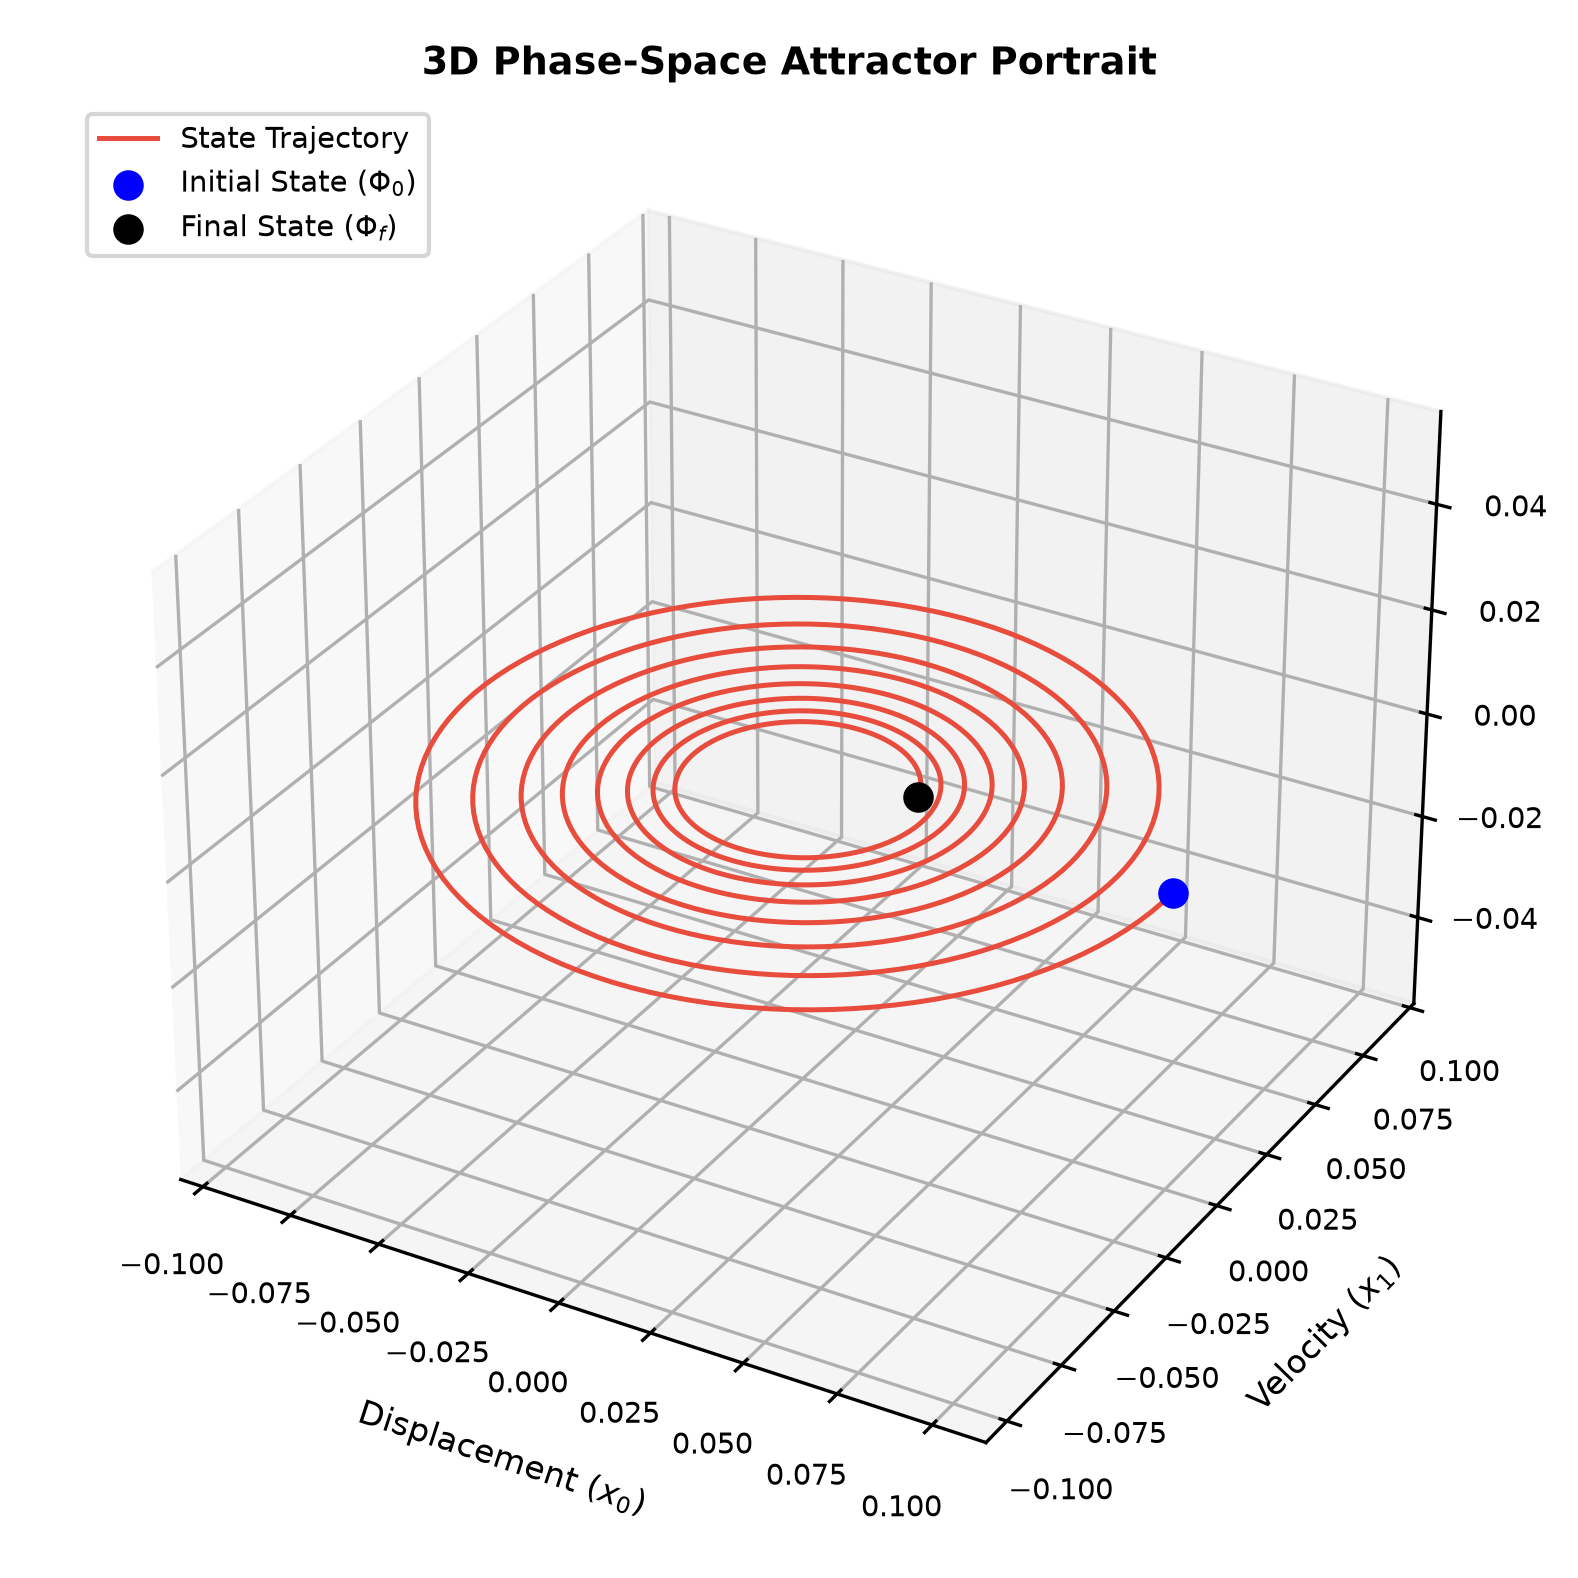
\includegraphics[width=0.5\textwidth]{contents/non-linear-oscillators/the-duffing-oscillator/phase_space_trajectory}
    \caption{3D Phase Space Trajectory of the Duffing Oscillator showing multi-well potential looping.}
    \label{fig:duffing_phase}
\end{figure}

\section{2D Evolution Plot}
\begin{figure}[h]
    \centering
    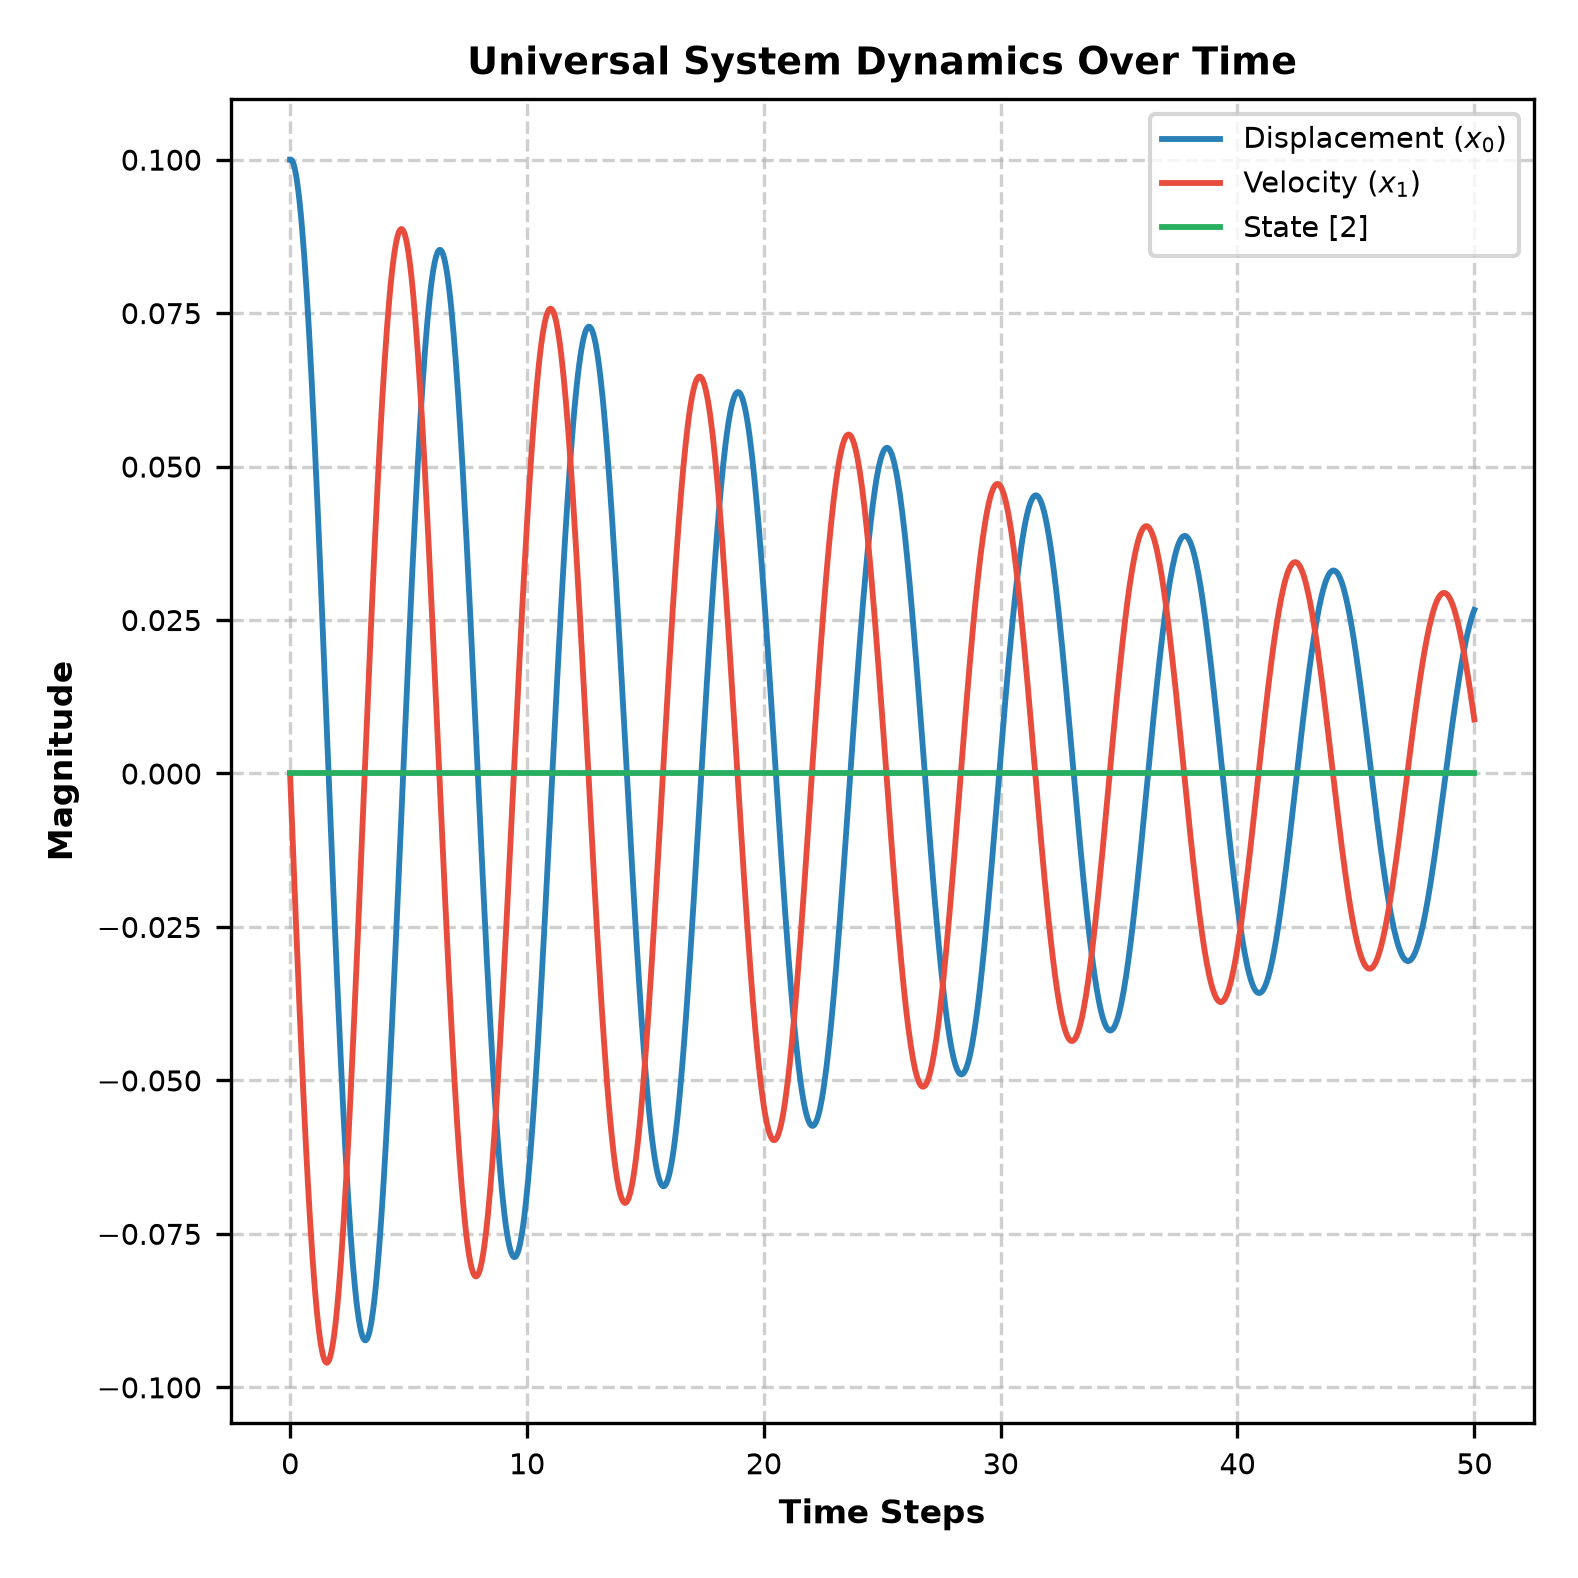
\includegraphics[width=0.5\textwidth]{contents/non-linear-oscillators/the-duffing-oscillator/system_evolution}
    \caption{2D System Evolution displaying driven harmonic displacement and velocity waveforms over time.}
    \label{fig:duffing_evolution}
\end{figure}
\clearpage
\section{Analysis of the Output}
The SDCM solver correctly maps the interplay between the double-well potential and external periodic forcing. The trajectory captures complex basin boundary transitions and periodic orbit entrapment without numerical instability.

\section{Conclusion}
The Duffing oscillator model highlights the strength of the SDCM framework in resolving cubic non-linearities and forced mechanical resonance phenomena.